% Author: Izaak Neutelings (March 2019)
% Inspiration: https://tex.stackexchange.com/questions/203597/automatically-generate-graphics-which-shows-light-diffusion-on-a-rough-surface
\documentclass[border=3pt,tikz]{standalone}
\usetikzlibrary{decorations.pathmorphing,decorations.markings,calc} % for random steps & snake
\usetikzlibrary{arrows.meta} % for arrow size
\tikzset{>=latex} % for LaTeX arrow head
\tikzstyle{radiation}=[-{Latex[length=1.5,width=1.2]},red!95!black!50,opacity=0.7,very thin,decorate,
                       decoration={snake,amplitude=0.7,segment length=2,post length=2}]

\begin{document}


% BLACK BODY
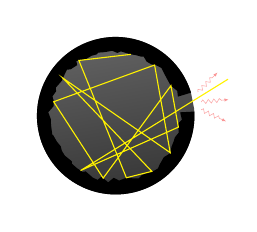
\begin{tikzpicture}[scale=1,rotate=10]
  
  \shade[top color=black!60,bottom color=black!80,shading angle=10] % background
    (7:1) arc (7:355:1);
  
  \fill[thick,black,postaction=decorate, % rough inner surface
    decoration={markings,mark=between positions 0.55 and 1 step 0.03 with {
                  \node[transform shape,inner sep=1pt]
                  (hit\pgfkeysvalueof{/pgf/decoration/mark info/sequence number}) {};
    }}]
    (7:1) arc (7:353:1) --++ (-7:-0.18)
    decorate[decoration={random steps,segment length=2,amplitude=1pt}]
        {arc (-7:-353:0.82)} -- cycle;
  
  \draw[yellow] % connect light ray to random points
    (8:1.5) -- (hit6.center) -- (hit1.center) -- (hit15.center) -- (hit5.center) --
    (hit9.center) -- (hit14.center) -- (hit2.center) -- (hit10.center) -- (hit3.center) --
    (hit4.center) -- (hit11.center) -- (hit13.center);
  
  \foreach \ang in {-35,-5,35}{
    \draw[radiation] (1,0)++(\ang:0.1 and 0.2) --++ (\ang:0.35);
  }

\end{tikzpicture}


% BLACK BODY - without infalling light
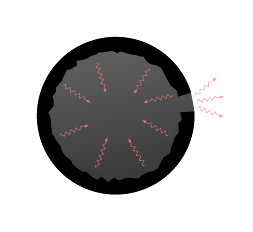
\begin{tikzpicture}[scale=1,rotate=10]
  
  \shade[top color=black!60,bottom color=black!80,shading angle=10] % background
    (7:1) arc (7:355:1);
  
  \fill[thick,black,postaction=decorate, % rough inner surface
    decoration={markings,mark=between positions 0.55 and 1 step 0.03 with {
                  \node[transform shape,inner sep=1pt]
                  (hit\pgfkeysvalueof{/pgf/decoration/mark info/sequence number}) {};
    }}]
    (7:1) arc (7:353:1) --++ (-7:-0.18)
    decorate[decoration={random steps,segment length=2,amplitude=1pt}]
        {arc (-7:-353:0.82)} -- cycle;
  
  \foreach \ang [evaluate={\angin=\ang-180+10*rand; \r=0.76+0.05*rand; \l=0.4+0.02*rand}] in {10,45,100,140,190,240,290,330}{
    \draw[radiation] (\ang:\r) --++ (\angin:\l);
  }
  
  \foreach \ang in {-30,0,30}{
    \draw[radiation] (1,0)++(\ang:0.05 and 0.16) --++ (\ang:0.35);
  }

\end{tikzpicture}


\end{document}
